% Prime counting: pi(x) against x/ln x and Li(x). Data from a short sieve
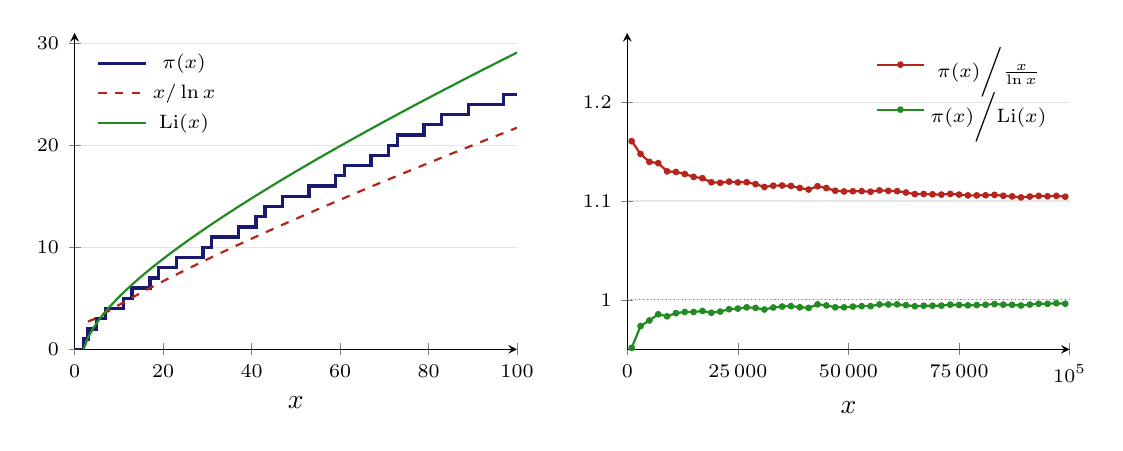
\begin{tikzpicture}
\begin{axis}[name=L,width=7.2cm,height=5.6cm,xmin=0,xmax=100,ymin=0,ymax=31,axis lines=left,
    xlabel={$x$},legend pos=north west,legend style={font=\scriptsize,draw=none,fill=none},
    ymajorgrids,grid style={gray!20},tick label style={font=\scriptsize}]
  \addplot[very thick,MidnightBlue] coordinates {(0,0) (2,0) (2,1) (3,1) (3,2) (5,2) (5,3) (7,3) (7,4) (11,4) (11,5) (13,5) (13,6) (17,6) (17,7) (19,7) (19,8) (23,8) (23,9) (29,9) (29,10) (31,10) (31,11) (37,11) (37,12) (41,12) (41,13) (43,13) (43,14) (47,14) (47,15) (53,15) (53,16) (59,16) (59,17) (61,17) (61,18) (67,18) (67,19) (71,19) (71,20) (73,20) (73,21) (79,21) (79,22) (83,22) (83,23) (89,23) (89,24) (97,24) (97,25) (100,25)};
  \addlegendentry{$\pi(x)$}
  \addplot[thick,BrickRed,dashed] coordinates {(3,2.731) (4,2.885) (5,3.107) (6,3.349) (7,3.597) (8,3.847) (9,4.096) (10,4.343) (11,4.587) (12,4.829) (13,5.068) (14,5.305) (15,5.539) (16,5.771) (17,6.000) (18,6.228) (19,6.453) (20,6.676) (21,6.898) (22,7.117) (23,7.335) (24,7.552) (25,7.767) (26,7.980) (27,8.192) (28,8.403) (29,8.612) (30,8.820) (31,9.027) (32,9.233) (33,9.438) (34,9.642) (35,9.844) (36,10.046) (37,10.247) (38,10.446) (39,10.645) (40,10.843) (41,11.041) (42,11.237) (43,11.433) (44,11.627) (45,11.821) (46,12.015) (47,12.207) (48,12.399) (49,12.591) (50,12.781) (51,12.971) (52,13.160) (53,13.349) (54,13.537) (55,13.725) (56,13.912) (57,14.098) (58,14.284) (59,14.470) (60,14.654) (61,14.839) (62,15.023) (63,15.206) (64,15.389) (65,15.571) (66,15.753) (67,15.935) (68,16.116) (69,16.296) (70,16.476) (71,16.656) (72,16.836) (73,17.014) (74,17.193) (75,17.371) (76,17.549) (77,17.726) (78,17.903) (79,18.080) (80,18.256) (81,18.432) (82,18.608) (83,18.783) (84,18.958) (85,19.133) (86,19.307) (87,19.481) (88,19.655) (89,19.828) (90,20.001) (91,20.174) (92,20.346) (93,20.518) (94,20.690) (95,20.861) (96,21.033) (97,21.204) (98,21.374) (99,21.545) (100,21.715)};
  \addlegendentry{$x/\ln x$}
  \addplot[thick,ForestGreen] coordinates {(2,0.000) (3,1.118) (4,1.922) (5,2.589) (6,3.177) (7,3.712) (8,4.209) (9,4.676) (10,5.120) (11,5.546) (12,5.955) (13,6.351) (14,6.736) (15,7.110) (16,7.475) (17,7.831) (18,8.181) (19,8.523) (20,8.860) (21,9.191) (22,9.517) (23,9.838) (24,10.155) (25,10.468) (26,10.777) (27,11.082) (28,11.383) (29,11.682) (30,11.977) (31,12.270) (32,12.560) (33,12.847) (34,13.132) (35,13.414) (36,13.695) (37,13.973) (38,14.248) (39,14.522) (40,14.794) (41,15.065) (42,15.333) (43,15.600) (44,15.865) (45,16.128) (46,16.390) (47,16.651) (48,16.910) (49,17.167) (50,17.424) (51,17.679) (52,17.932) (53,18.185) (54,18.436) (55,18.686) (56,18.935) (57,19.183) (58,19.430) (59,19.676) (60,19.920) (61,20.164) (62,20.407) (63,20.649) (64,20.890) (65,21.130) (66,21.369) (67,21.607) (68,21.844) (69,22.081) (70,22.317) (71,22.552) (72,22.786) (73,23.019) (74,23.252) (75,23.484) (76,23.715) (77,23.946) (78,24.176) (79,24.405) (80,24.633) (81,24.861) (82,25.089) (83,25.315) (84,25.541) (85,25.767) (86,25.991) (87,26.216) (88,26.439) (89,26.662) (90,26.885) (91,27.107) (92,27.328) (93,27.549) (94,27.769) (95,27.989) (96,28.209) (97,28.427) (98,28.646) (99,28.864) (100,29.081)};
  \addlegendentry{$\mathrm{Li}(x)$}
\end{axis}
\begin{axis}[at={(L.east)},anchor=west,xshift=1.4cm,width=7.2cm,height=5.6cm,xmin=0,xmax=100000,ymin=0.95,ymax=1.27,
    axis lines=left,xlabel={$x$},scaled x ticks=false,xtick={0,25000,50000,75000,100000},
    xticklabels={$0$,$25\,000$,$50\,000$,$75\,000$,$10^5$},
    legend style={at={(0.98,0.99)},anchor=north east,font=\scriptsize,draw=none,fill=none},
    ymajorgrids,grid style={gray!20},tick label style={font=\scriptsize}]
  \addplot[thick,BrickRed,mark=*,mark size=0.8pt] coordinates {(1000,1.1605) (3000,1.1476) (5000,1.1396) (7000,1.1383) (9000,1.1300) (11000,1.1294) (13000,1.1273) (15000,1.1244) (17000,1.1231) (19000,1.1190) (21000,1.1184) (23000,1.1196) (25000,1.1188) (27000,1.1190) (29000,1.1171) (31000,1.1142) (33000,1.1155) (35000,1.1157) (37000,1.1153) (39000,1.1132) (41000,1.1116) (43000,1.1150) (45000,1.1131) (47000,1.1104) (49000,1.1097) (51000,1.1099) (53000,1.1100) (55000,1.1094) (57000,1.1108) (59000,1.1103) (61000,1.1100) (63000,1.1086) (65000,1.1070) (67000,1.1071) (69000,1.1068) (71000,1.1065) (73000,1.1072) (75000,1.1065) (77000,1.1057) (79000,1.1057) (81000,1.1058) (83000,1.1062) (85000,1.1053) (87000,1.1047) (89000,1.1037) (91000,1.1045) (93000,1.1052) (95000,1.1048) (97000,1.1052) (99000,1.1044)};
  \addlegendentry{$\pi(x)\big/\frac x{\ln x}$}
  \addplot[thick,ForestGreen,mark=*,mark size=0.8pt] coordinates {(1000,0.9515) (3000,0.9735) (5000,0.9792) (7000,0.9855) (9000,0.9834) (11000,0.9866) (13000,0.9878) (15000,0.9878) (17000,0.9888) (19000,0.9870) (21000,0.9882) (23000,0.9906) (25000,0.9912) (27000,0.9925) (29000,0.9919) (31000,0.9903) (33000,0.9923) (35000,0.9933) (37000,0.9937) (39000,0.9926) (41000,0.9919) (43000,0.9955) (45000,0.9944) (47000,0.9925) (49000,0.9925) (51000,0.9932) (53000,0.9937) (55000,0.9937) (57000,0.9954) (59000,0.9954) (61000,0.9955) (63000,0.9947) (65000,0.9936) (67000,0.9941) (69000,0.9941) (71000,0.9942) (73000,0.9952) (75000,0.9949) (77000,0.9945) (79000,0.9948) (81000,0.9951) (83000,0.9958) (85000,0.9952) (87000,0.9950) (89000,0.9943) (91000,0.9953) (93000,0.9961) (95000,0.9960) (97000,0.9966) (99000,0.9961)};
  \addlegendentry{$\pi(x)\big/\mathrm{Li}(x)$}
  \draw[gray,densely dotted] (axis cs:0,1) -- (axis cs:100000,1);
\end{axis}
\end{tikzpicture}
